% Editable native annotations around unchanged verified IDE photographs.
\par
\begin{figure}[htbp]
\centering
\newsavebox{\MARSdeltasizessteadyBox}
\sbox{\MARSdeltasizessteadyBox}{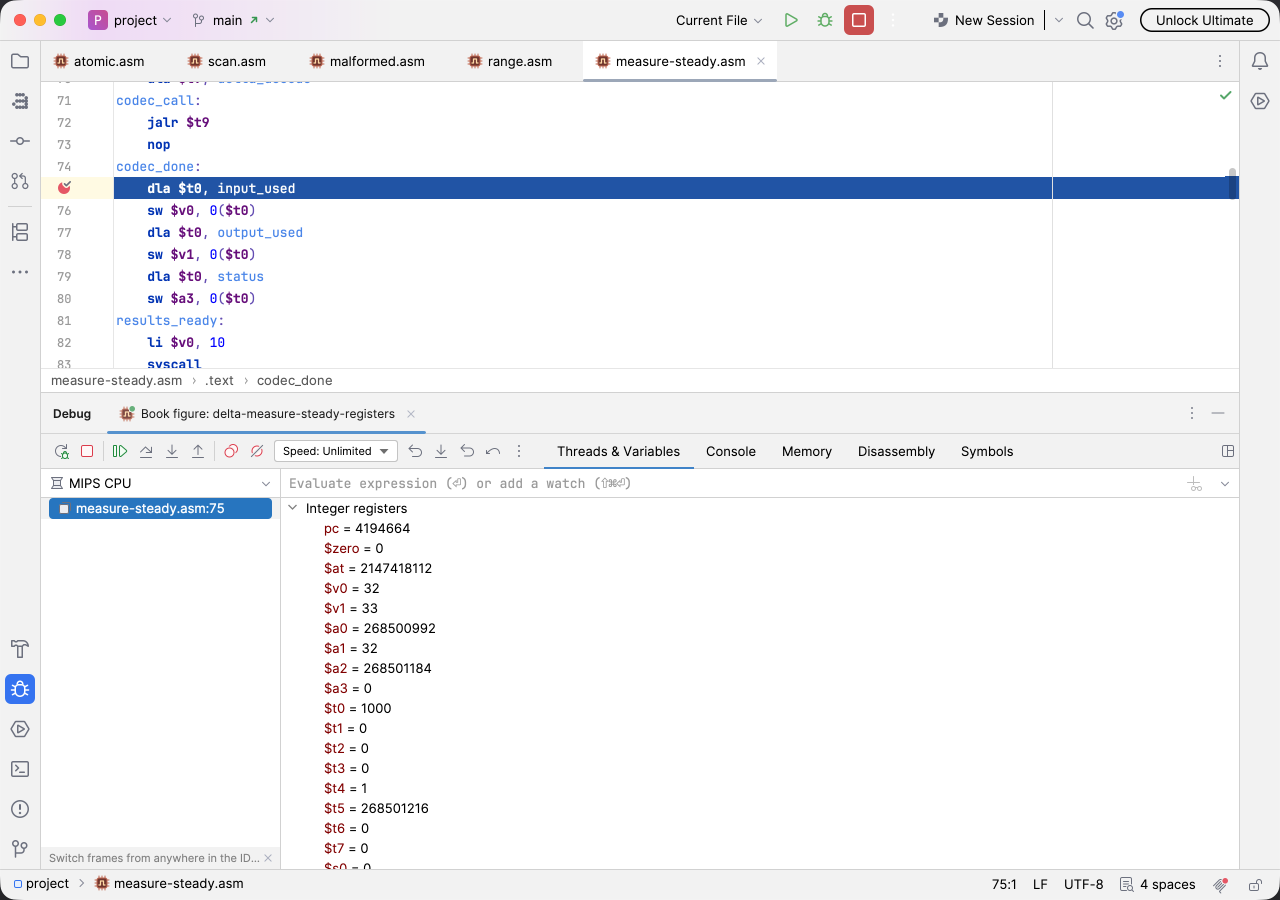
\includegraphics[artifact]{packages/023-delta-varint/captures/f04/steady.png}}
\newsavebox{\MARSdeltasizesrampBox}
\sbox{\MARSdeltasizesrampBox}{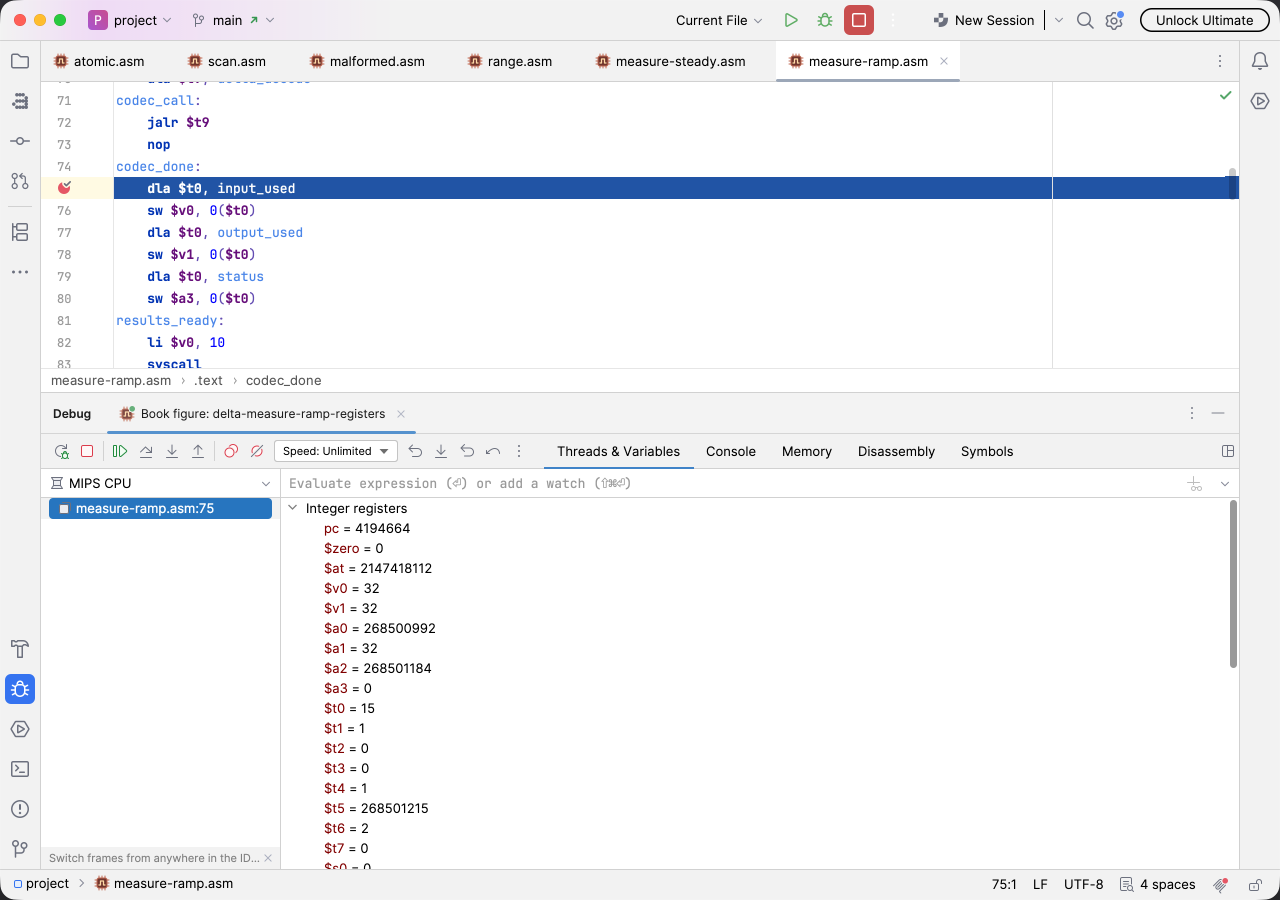
\includegraphics[artifact]{packages/023-delta-varint/captures/f04/ramp.png}}
\newsavebox{\MARSdeltasizestimestampsBox}
\sbox{\MARSdeltasizestimestampsBox}{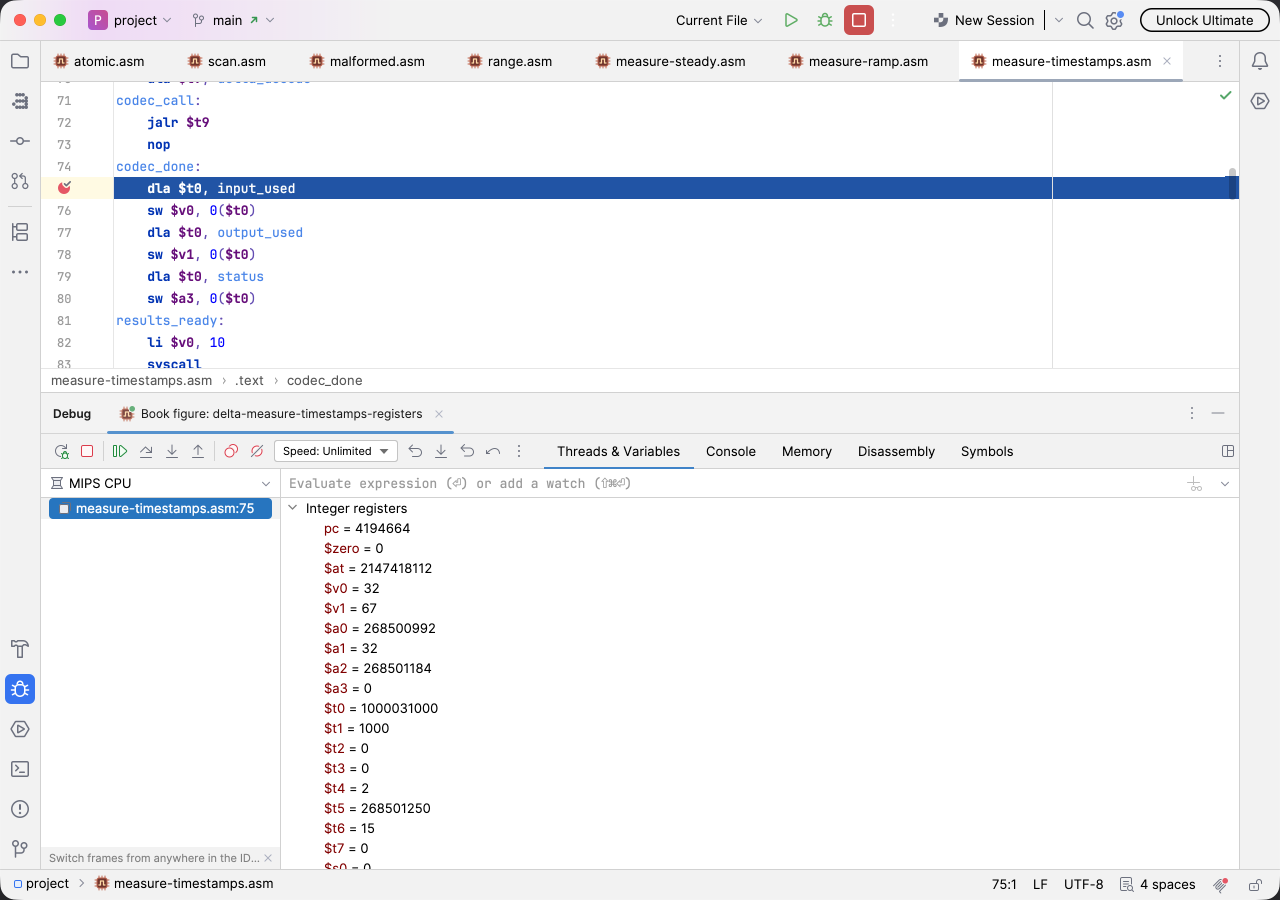
\includegraphics[artifact]{packages/023-delta-varint/captures/f04/timestamps.png}}
\newsavebox{\MARSdeltasizesspikeBox}
\sbox{\MARSdeltasizesspikeBox}{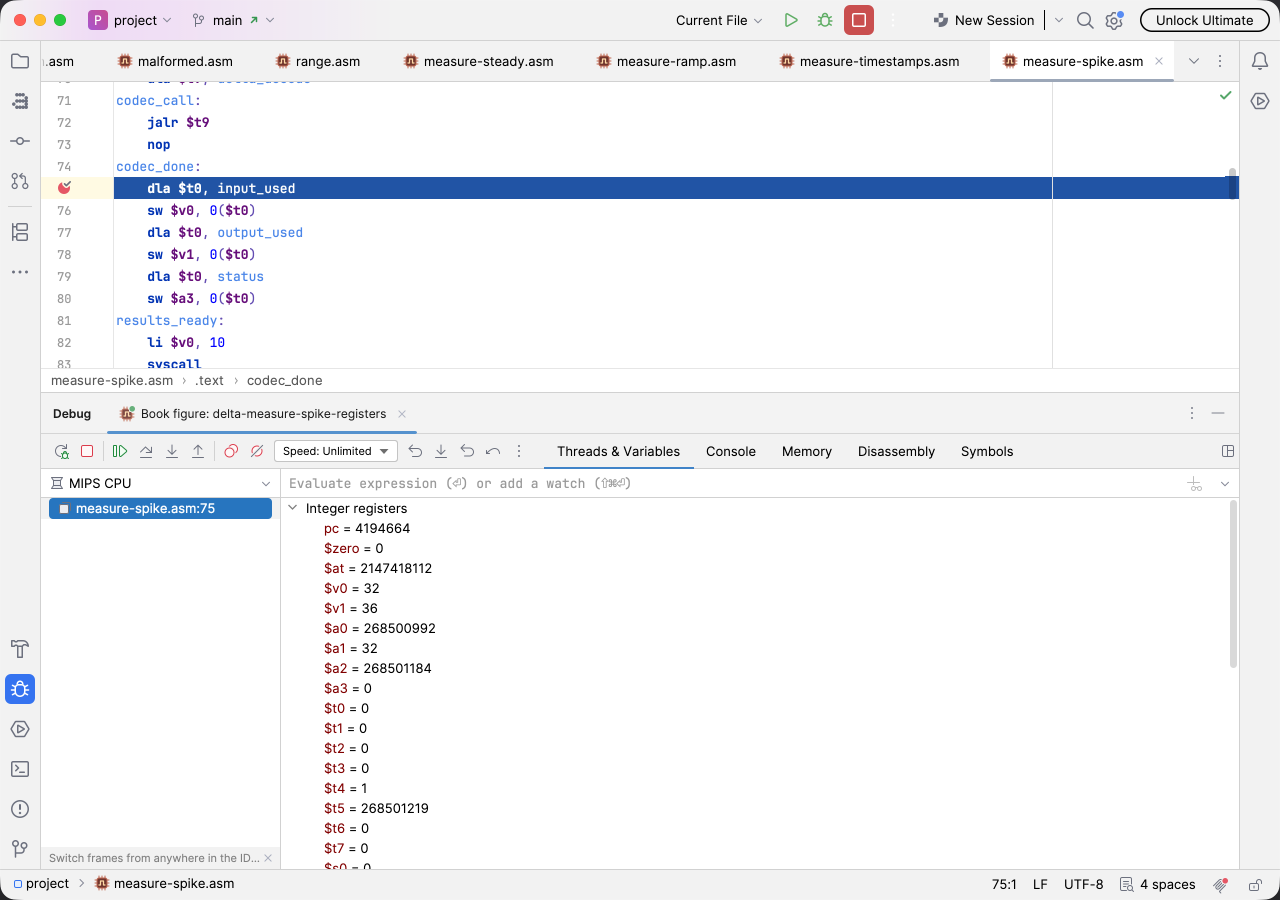
\includegraphics[artifact]{packages/023-delta-varint/captures/f04/spike.png}}
\newsavebox{\MARSdeltasizesextremesBox}
\sbox{\MARSdeltasizesextremesBox}{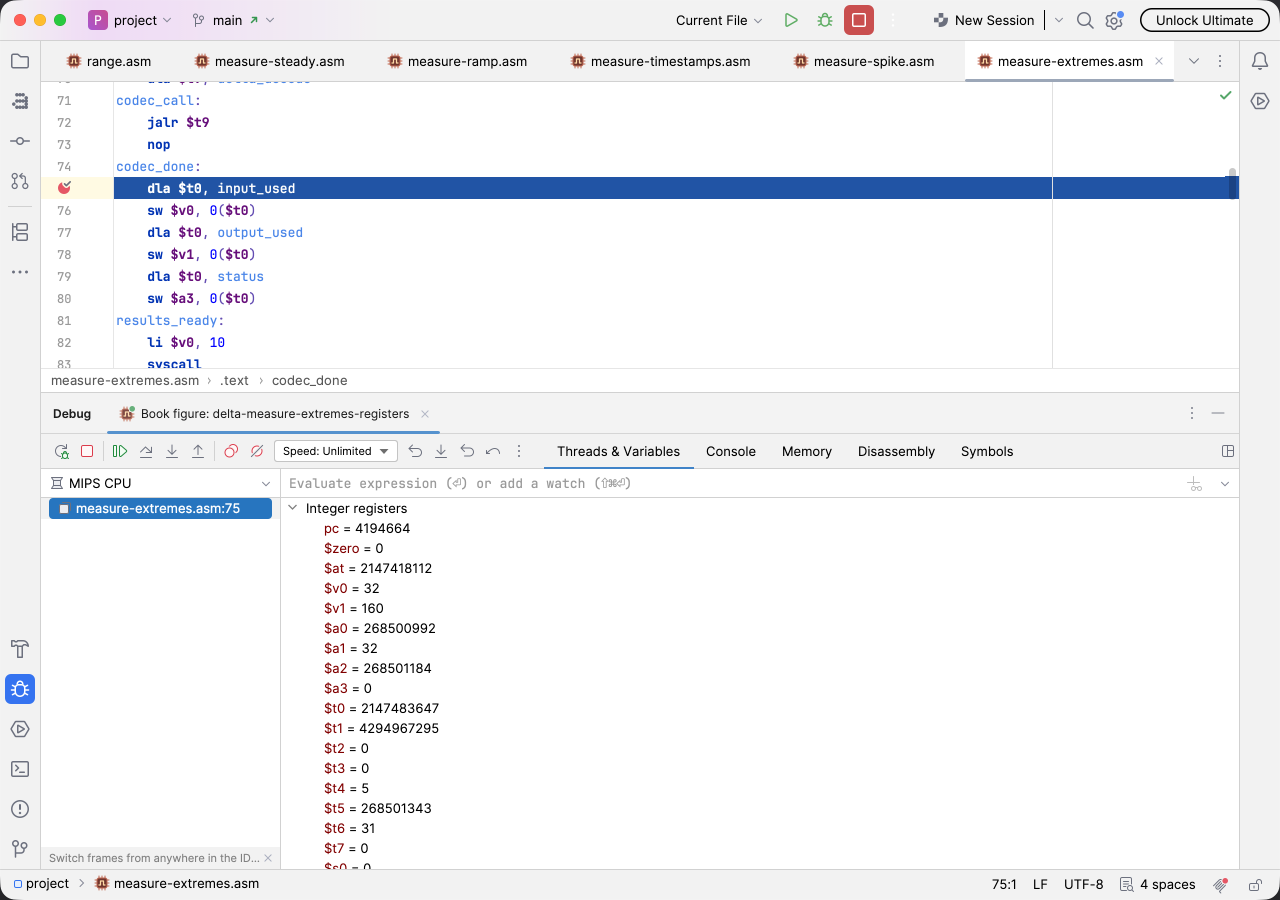
\includegraphics[artifact]{packages/023-delta-varint/captures/f04/extremes.png}}
\newsavebox{\MARSdeltasizesrandomBox}
\sbox{\MARSdeltasizesrandomBox}{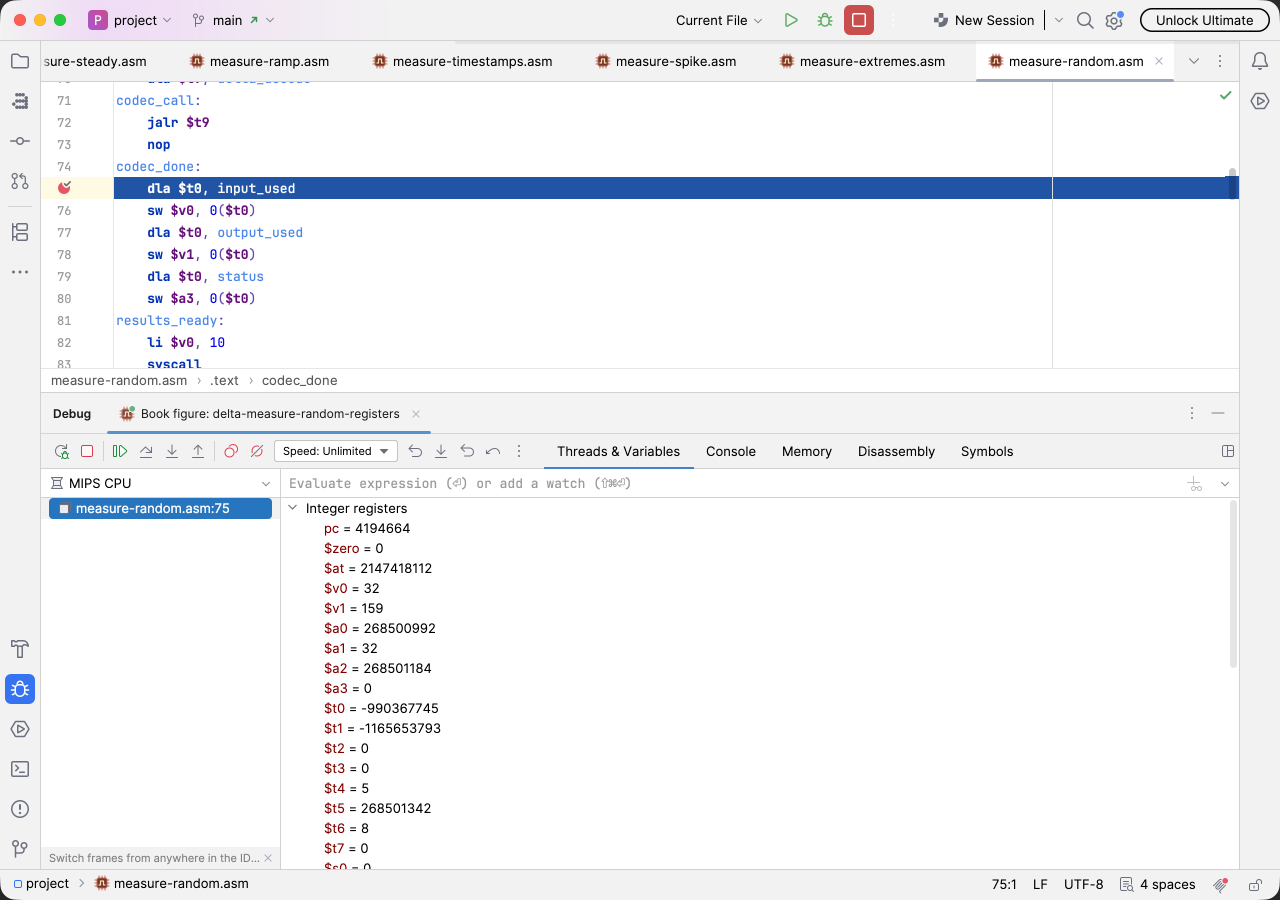
\includegraphics[artifact]{packages/023-delta-varint/captures/f04/random.png}}
\edef\MARSdeltasizessteadyLeft{\the\dimexpr0.246093750\wd\MARSdeltasizessteadyBox\relax}
\edef\MARSdeltasizessteadyBottom{\the\dimexpr0.312222222\ht\MARSdeltasizessteadyBox\relax}
\edef\MARSdeltasizessteadyRight{\the\dimexpr0.553906250\wd\MARSdeltasizessteadyBox\relax}
\edef\MARSdeltasizessteadyTop{\the\dimexpr0.640000000\ht\MARSdeltasizessteadyBox\relax}
\edef\MARSdeltasizesrampLeft{\the\dimexpr0.246093750\wd\MARSdeltasizesrampBox\relax}
\edef\MARSdeltasizesrampBottom{\the\dimexpr0.312222222\ht\MARSdeltasizesrampBox\relax}
\edef\MARSdeltasizesrampRight{\the\dimexpr0.553906250\wd\MARSdeltasizesrampBox\relax}
\edef\MARSdeltasizesrampTop{\the\dimexpr0.640000000\ht\MARSdeltasizesrampBox\relax}
\edef\MARSdeltasizestimestampsLeft{\the\dimexpr0.246093750\wd\MARSdeltasizestimestampsBox\relax}
\edef\MARSdeltasizestimestampsBottom{\the\dimexpr0.312222222\ht\MARSdeltasizestimestampsBox\relax}
\edef\MARSdeltasizestimestampsRight{\the\dimexpr0.553906250\wd\MARSdeltasizestimestampsBox\relax}
\edef\MARSdeltasizestimestampsTop{\the\dimexpr0.640000000\ht\MARSdeltasizestimestampsBox\relax}
\edef\MARSdeltasizesspikeLeft{\the\dimexpr0.246093750\wd\MARSdeltasizesspikeBox\relax}
\edef\MARSdeltasizesspikeBottom{\the\dimexpr0.312222222\ht\MARSdeltasizesspikeBox\relax}
\edef\MARSdeltasizesspikeRight{\the\dimexpr0.553906250\wd\MARSdeltasizesspikeBox\relax}
\edef\MARSdeltasizesspikeTop{\the\dimexpr0.640000000\ht\MARSdeltasizesspikeBox\relax}
\edef\MARSdeltasizesextremesLeft{\the\dimexpr0.246093750\wd\MARSdeltasizesextremesBox\relax}
\edef\MARSdeltasizesextremesBottom{\the\dimexpr0.312222222\ht\MARSdeltasizesextremesBox\relax}
\edef\MARSdeltasizesextremesRight{\the\dimexpr0.553906250\wd\MARSdeltasizesextremesBox\relax}
\edef\MARSdeltasizesextremesTop{\the\dimexpr0.640000000\ht\MARSdeltasizesextremesBox\relax}
\edef\MARSdeltasizesrandomLeft{\the\dimexpr0.246093750\wd\MARSdeltasizesrandomBox\relax}
\edef\MARSdeltasizesrandomBottom{\the\dimexpr0.312222222\ht\MARSdeltasizesrandomBox\relax}
\edef\MARSdeltasizesrandomRight{\the\dimexpr0.553906250\wd\MARSdeltasizesrandomBox\relax}
\edef\MARSdeltasizesrandomTop{\the\dimexpr0.640000000\ht\MARSdeltasizesrandomBox\relax}
\begin{tikzpicture}[alt={Six native register details at codec_done show 32 committed readings per dataset. Encoded bytes are 33 steady, 32 ramp, 67 timestamps, 36 spike, 160 alternating signed endpoints and 159 seeded random. Status zero is checked for every call but is outside these cropped details. The text compares byte sizes separately from checked whole-function instruction work.}]
\node[anchor=north west,inner sep=0,font=\small\bfseries] (steady-title) at (6mm,0) {Steady readings};
\node[anchor=north west,inner sep=0] (steady) at ([yshift=-1mm]steady-title.south west) {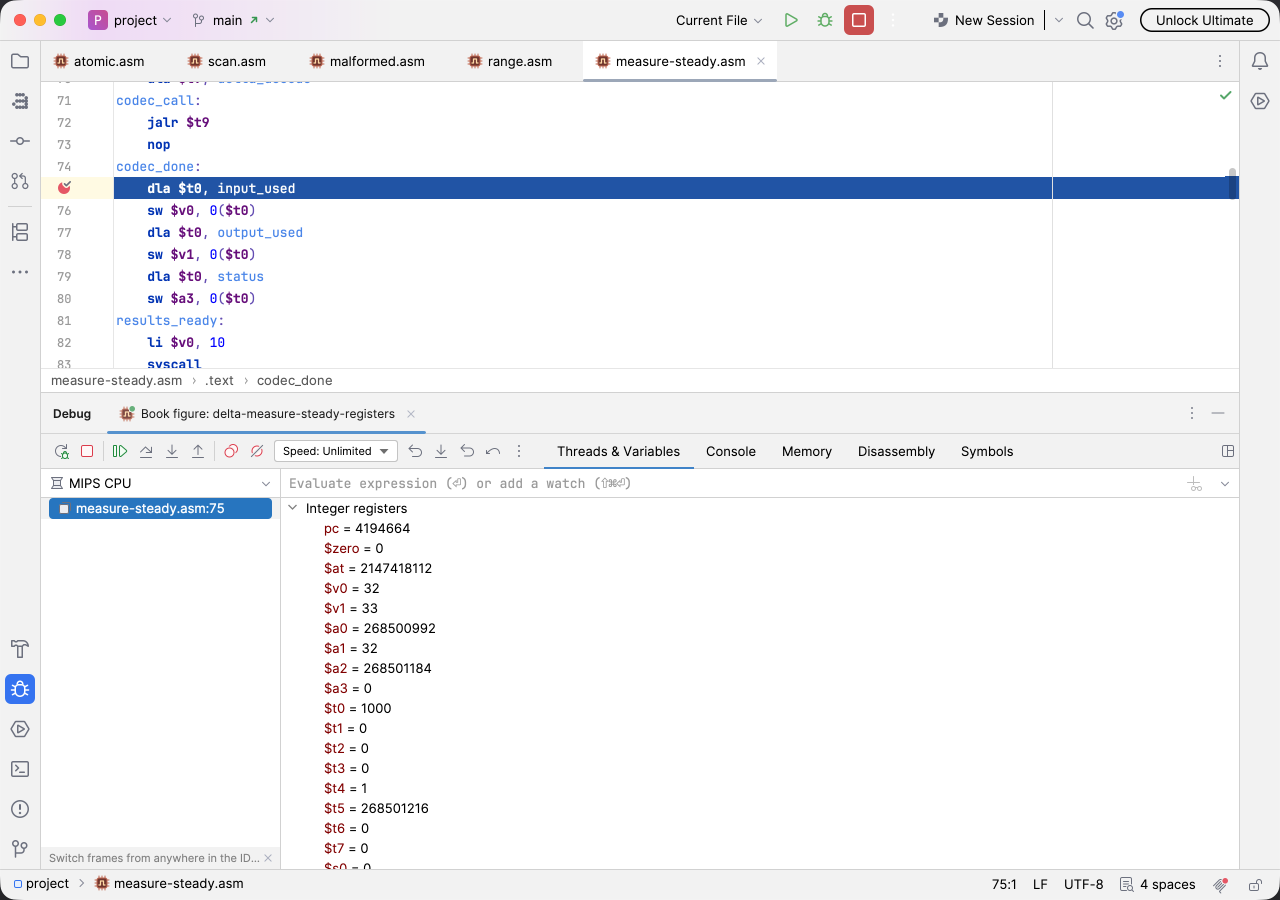
\includegraphics[width=0.42\linewidth,artifact,trim={\MARSdeltasizessteadyLeft{} \MARSdeltasizessteadyBottom{} \MARSdeltasizessteadyRight{} \MARSdeltasizessteadyTop{}},clip]{packages/023-delta-varint/captures/f04/steady.png}};
\begin{scope}[shift={(steady.south west)},x={($(steady.south east)-(steady.south west)$)},y={($(steady.north west)-(steady.south west)$)}]
\draw[black,line width=0.7pt] (0.023437500,0.023255814) rectangle (0.257812500,0.953488372);
\node[draw=black,fill=white,circle,inner sep=1.5pt,font=\footnotesize] at ($(0.023437500,0.953488372)+(-3mm,0)$) {1};
\end{scope}
\node[anchor=north west,inner sep=0,font=\small\bfseries] (ramp-title) at (0.55\linewidth,0 |- steady-title.north) {Ramp readings};
\node[anchor=north west,inner sep=0] (ramp) at ([yshift=-1mm]ramp-title.south west) {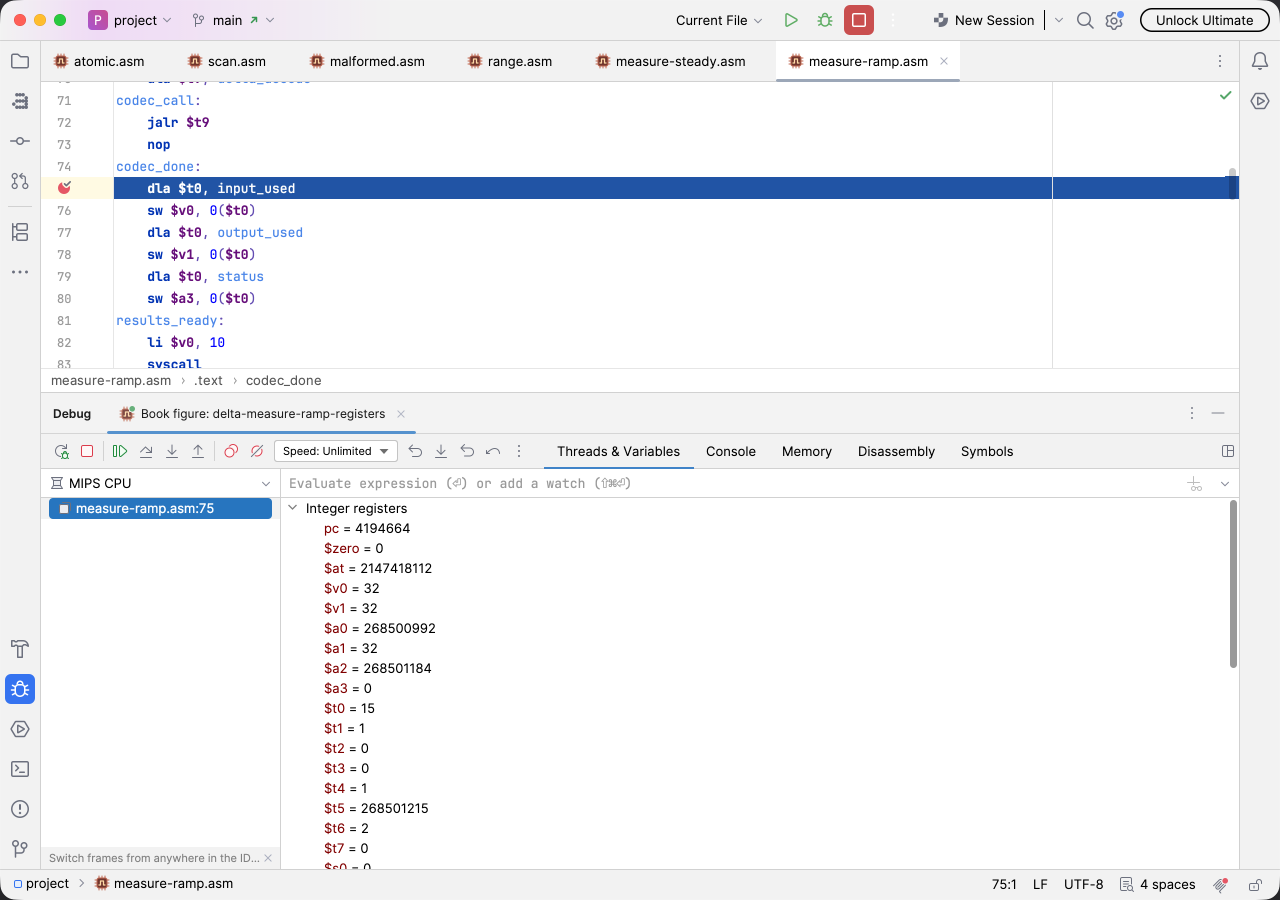
\includegraphics[width=0.42\linewidth,artifact,trim={\MARSdeltasizesrampLeft{} \MARSdeltasizesrampBottom{} \MARSdeltasizesrampRight{} \MARSdeltasizesrampTop{}},clip]{packages/023-delta-varint/captures/f04/ramp.png}};
\begin{scope}[shift={(ramp.south west)},x={($(ramp.south east)-(ramp.south west)$)},y={($(ramp.north west)-(ramp.south west)$)}]
\draw[black,line width=0.7pt] (0.023437500,0.023255814) rectangle (0.257812500,0.953488372);
\node[draw=black,fill=white,circle,inner sep=1.5pt,font=\footnotesize] at ($(0.023437500,0.953488372)+(-3mm,0)$) {2};
\end{scope}
\node[anchor=north west,inner sep=0,font=\small\bfseries] (timestamps-title) at ([yshift=-1mm]steady.south west) {Timestamp readings};
\node[anchor=north west,inner sep=0] (timestamps) at ([yshift=-1mm]timestamps-title.south west) {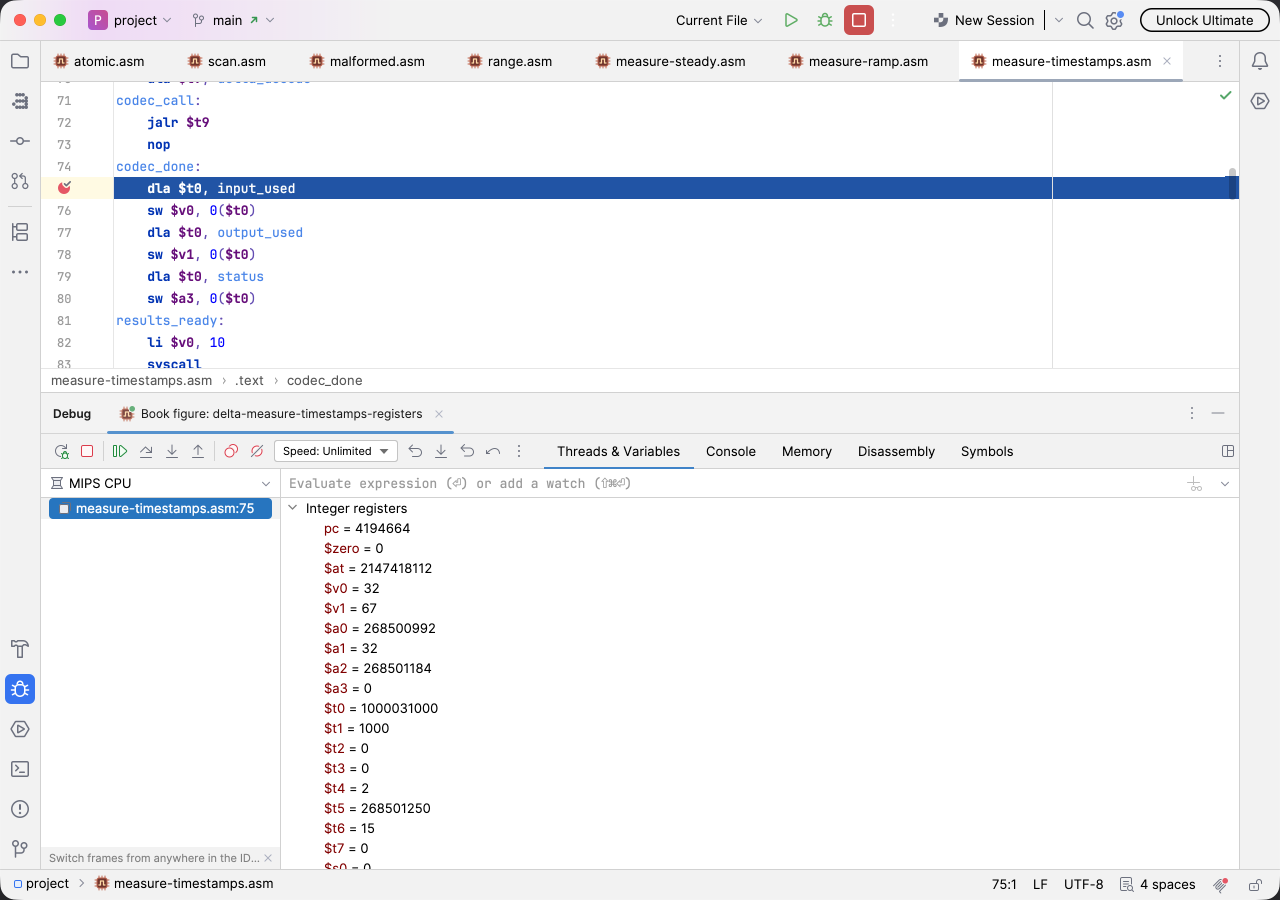
\includegraphics[width=0.42\linewidth,artifact,trim={\MARSdeltasizestimestampsLeft{} \MARSdeltasizestimestampsBottom{} \MARSdeltasizestimestampsRight{} \MARSdeltasizestimestampsTop{}},clip]{packages/023-delta-varint/captures/f04/timestamps.png}};
\begin{scope}[shift={(timestamps.south west)},x={($(timestamps.south east)-(timestamps.south west)$)},y={($(timestamps.north west)-(timestamps.south west)$)}]
\draw[black,line width=0.7pt] (0.023437500,0.023255814) rectangle (0.257812500,0.953488372);
\node[draw=black,fill=white,circle,inner sep=1.5pt,font=\footnotesize] at ($(0.023437500,0.953488372)+(-3mm,0)$) {3};
\end{scope}
\node[anchor=north west,inner sep=0,font=\small\bfseries] (spike-title) at (0.55\linewidth,0 |- timestamps-title.north) {Single spike};
\node[anchor=north west,inner sep=0] (spike) at ([yshift=-1mm]spike-title.south west) {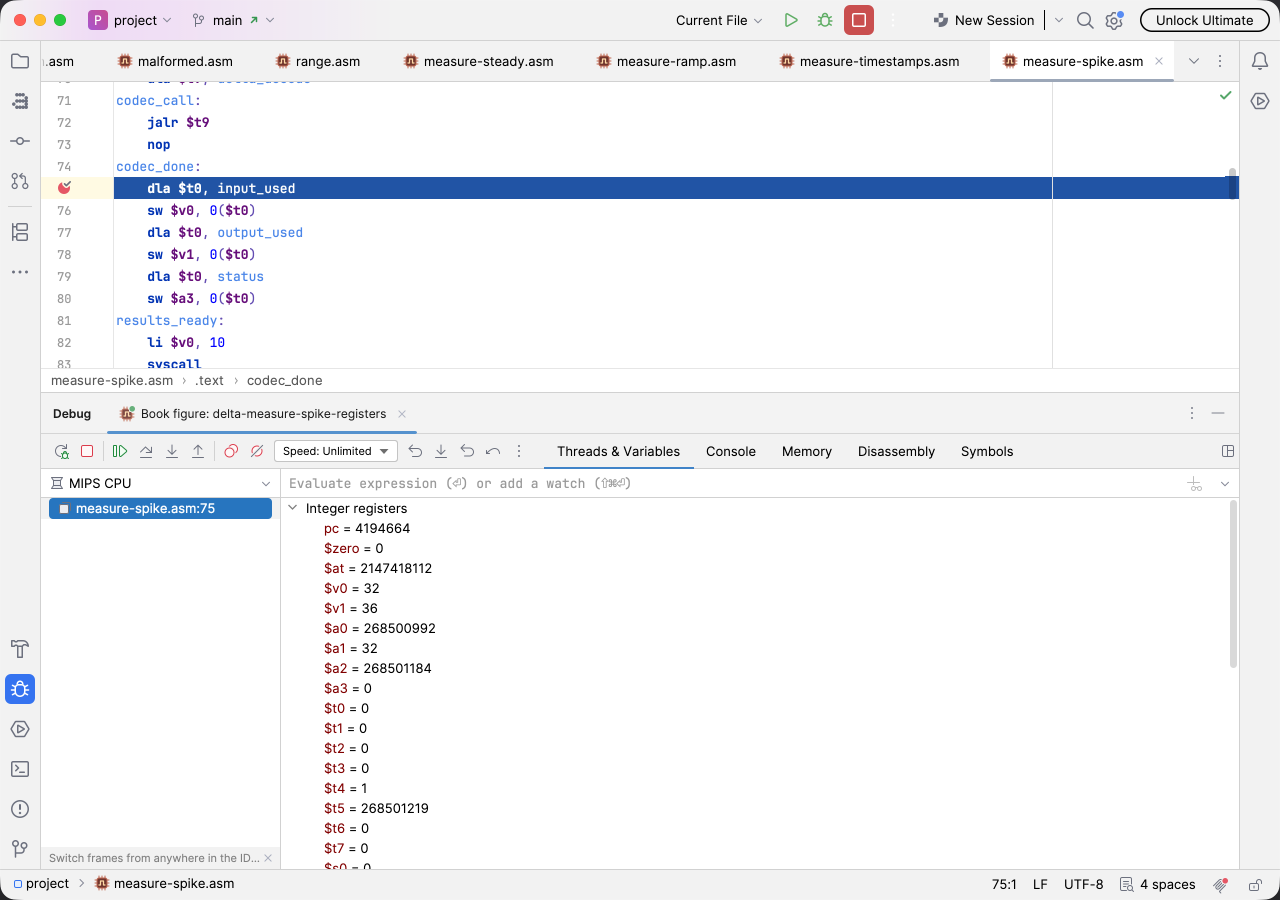
\includegraphics[width=0.42\linewidth,artifact,trim={\MARSdeltasizesspikeLeft{} \MARSdeltasizesspikeBottom{} \MARSdeltasizesspikeRight{} \MARSdeltasizesspikeTop{}},clip]{packages/023-delta-varint/captures/f04/spike.png}};
\begin{scope}[shift={(spike.south west)},x={($(spike.south east)-(spike.south west)$)},y={($(spike.north west)-(spike.south west)$)}]
\draw[black,line width=0.7pt] (0.023437500,0.023255814) rectangle (0.257812500,0.953488372);
\node[draw=black,fill=white,circle,inner sep=1.5pt,font=\footnotesize] at ($(0.023437500,0.953488372)+(-3mm,0)$) {4};
\end{scope}
\node[anchor=north west,inner sep=0,font=\small\bfseries] (extremes-title) at ([yshift=-1mm]timestamps.south west) {Alternating signed endpoints};
\node[anchor=north west,inner sep=0] (extremes) at ([yshift=-1mm]extremes-title.south west) {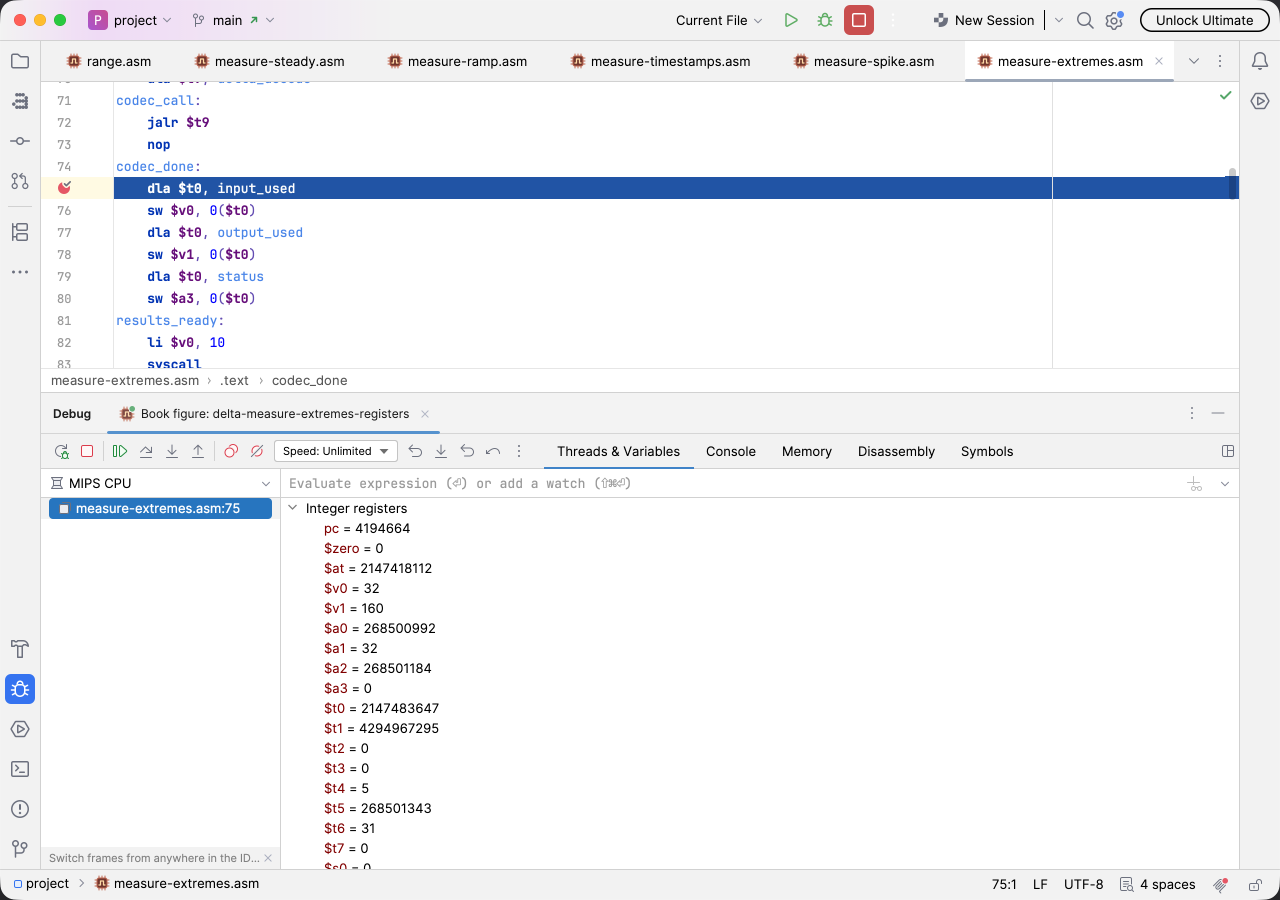
\includegraphics[width=0.42\linewidth,artifact,trim={\MARSdeltasizesextremesLeft{} \MARSdeltasizesextremesBottom{} \MARSdeltasizesextremesRight{} \MARSdeltasizesextremesTop{}},clip]{packages/023-delta-varint/captures/f04/extremes.png}};
\begin{scope}[shift={(extremes.south west)},x={($(extremes.south east)-(extremes.south west)$)},y={($(extremes.north west)-(extremes.south west)$)}]
\draw[black,line width=0.7pt] (0.023437500,0.023255814) rectangle (0.273437500,0.953488372);
\node[draw=black,fill=white,circle,inner sep=1.5pt,font=\footnotesize] at ($(0.023437500,0.953488372)+(-3mm,0)$) {5};
\end{scope}
\node[anchor=north west,inner sep=0,font=\small\bfseries] (random-title) at (0.55\linewidth,0 |- extremes-title.north) {Seeded random words};
\node[anchor=north west,inner sep=0] (random) at ([yshift=-1mm]random-title.south west) {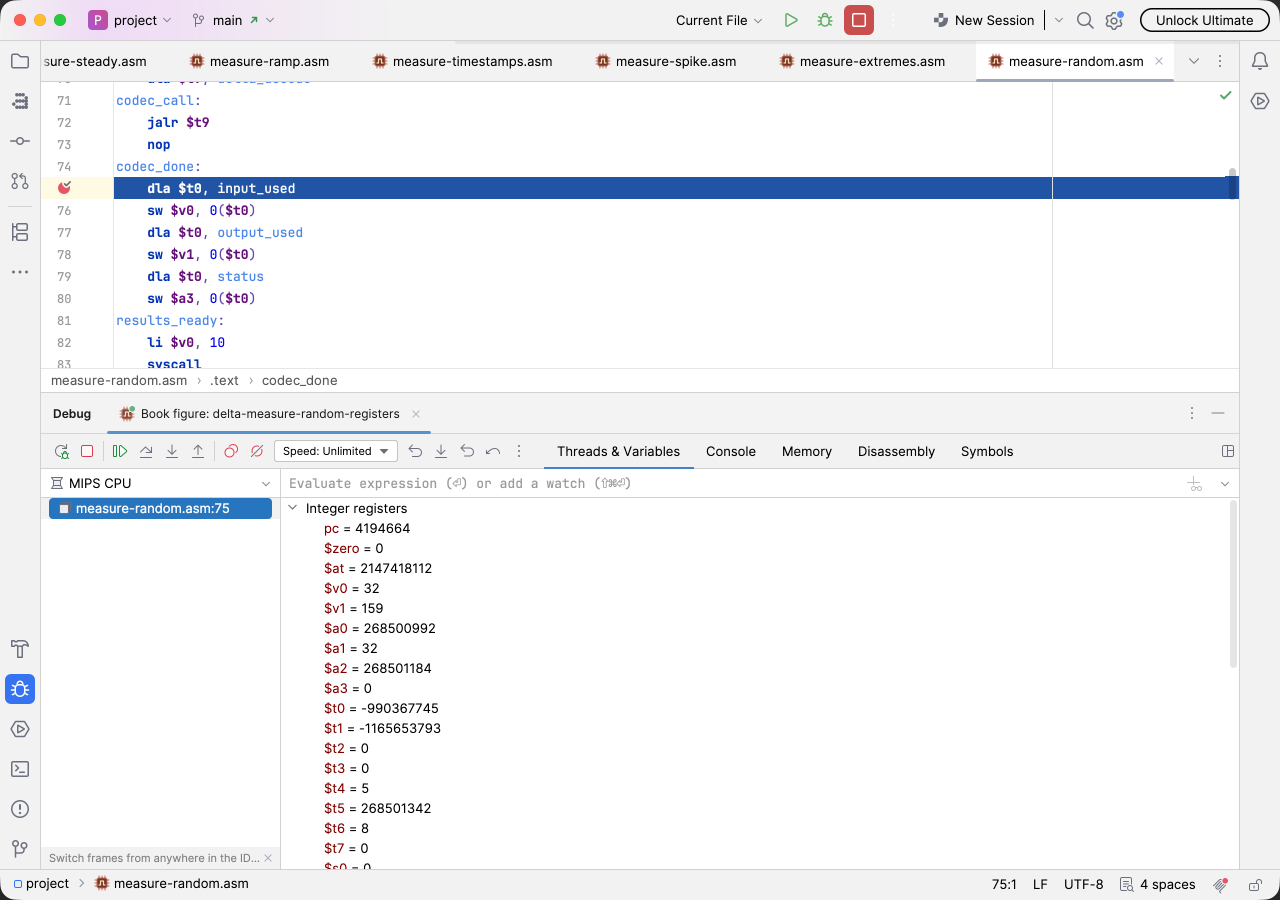
\includegraphics[width=0.42\linewidth,artifact,trim={\MARSdeltasizesrandomLeft{} \MARSdeltasizesrandomBottom{} \MARSdeltasizesrandomRight{} \MARSdeltasizesrandomTop{}},clip]{packages/023-delta-varint/captures/f04/random.png}};
\begin{scope}[shift={(random.south west)},x={($(random.south east)-(random.south west)$)},y={($(random.north west)-(random.south west)$)}]
\draw[black,line width=0.7pt] (0.023437500,0.023255814) rectangle (0.273437500,0.953488372);
\node[draw=black,fill=white,circle,inner sep=1.5pt,font=\footnotesize] at ($(0.023437500,0.953488372)+(-3mm,0)$) {6};
\end{scope}
\end{tikzpicture}
\par\smallskip
\begin{minipage}{\linewidth}
\small
\begin{enumerate}
\setlength{\itemsep}{2pt}
\setlength{\parsep}{0pt}
\item Steady 1000 returns 32 readings and 33 bytes, with status zero. The first reading needs two bytes; each later zero delta needs one. Independent mapping needs 64 bytes and fixed words need 128. Checked encoder instruction totals are 1041 for this implementation and 1072 for the alternative.
\item The ramp returns 32 bytes. Its original values already fit one-byte mapped forms, so subtraction saves no bytes relative to independent mapping. The checked instruction totals are 1026 and 1062.
\item Timestamps return 67 bytes, compared with 160 for independently mapped readings. The first large timestamp costs five bytes; 31 changes of 1000 cost two bytes each. The checked instruction totals are 1551 and 1546.
\item The single spike returns 36 bytes, compared with 34 for independent mapping. Both the upward and downward changes cost extra bytes. The checked instruction totals are 1086 and 1120.
\item Alternating signed endpoints return 160 bytes, exceeding the 128-byte fixed-width input. Every delta needs five bytes. The checked instruction totals are 2946 and 2850.
\item Seeded random words return 159 bytes, also exceeding fixed-width storage. The checked instruction totals are 2931 and 2840. Instruction counts come from separate complete-function observations; these register views show committed units and status, not elapsed time.
\end{enumerate}
\end{minipage}
\caption{Six completed encoder calls return different byte counts for the same number of readings.}
\label{capture:023-delta-varint-f04}
\label{delta-f04}
\end{figure}
\par
